\documentclass[10pt ]{article}

\usepackage{times}
\usepackage{epsfig}
\usepackage{graphicx}
\usepackage{amsmath}
\usepackage{amssymb}
\usepackage{amsthm}
\usepackage{hyperref}
\usepackage{soul}
\DeclareMathOperator*{\argmaxA}{arg\,max}

\newtheorem{example}{Example}

\usepackage{tikz}
\usepackage{soul}
\usetikzlibrary{shapes.misc, positioning, shapes.geometric, arrows}
%\usepackage[a4paper,margin=1cm,landscape]{geometry}
\usetikzlibrary{positioning,shapes,shadows}


\tikzstyle{conv2d} = [rectangle, rounded corners, minimum width=4cm, minimum height=1cm,text centered, draw=black, fill=green!30]
\tikzstyle{bn} = [rectangle, rounded corners, minimum width=4cm, minimum height=1cm,text centered, draw=black, fill=red!30]
\tikzstyle{relu} = [rectangle, rounded corners, minimum width=4cm, minimum height=1cm,text centered, draw=black, fill=blue!30]
\tikzstyle{add} = [circle, radius=1cm,text centered, draw=black]
\tikzstyle{arrow} = [thick,->,>=stealth]
\tikzstyle{downsample} = [rectangle, minimum width=6cm, minimum height=4cm,text centered, draw=black, fill=yellow!30]
\tikzstyle{maxpool} = [rectangle, rounded corners, minimum width=4cm, minimum height=1cm,text centered, draw=black, fill=gray!30]

\tikzstyle{btds} = [rectangle, rounded corners, minimum width=4cm, minimum height=1cm,text centered, draw=black, fill=orange!30]

\tikzstyle{btnods} = [rectangle, rounded corners, minimum width=4cm, minimum height=1cm,text centered, draw=black, fill=violet!30]

\def\ttx{1.4}

\setcounter{page}{1}
\begin{document}

\title{Estimating the parameters of a Mixture of Gaussians model}

\author{Mohsen Kiskani}

\maketitle

%\begin{abstract}
%\end{abstract}

\section{Problem definition}

We have a Mixture of Gaussians (MoG) model with parameters $\theta = (\pi_1, \mu_1, \sigma_1, \pi_2, \mu_2, \sigma_2)$. We want to estimate the parameter vector $\theta$ using the data $y_{1:N}$.
We assume that each data point is gathered independently according to the following distribution
\begin{align}
P(y \mid \theta) = \pi_1 \frac{1}{\sigma_1 \sqrt{2 \pi}} \exp \left( -\frac{(y-\mu_1)^2}{2\sigma_1^2}\right) + \pi_2 \frac{1}{\sigma_2 \sqrt{2 \pi}} \exp \left( -\frac{(y-\mu_2)^2}{2\sigma_2^2}\right) 
\end{align}
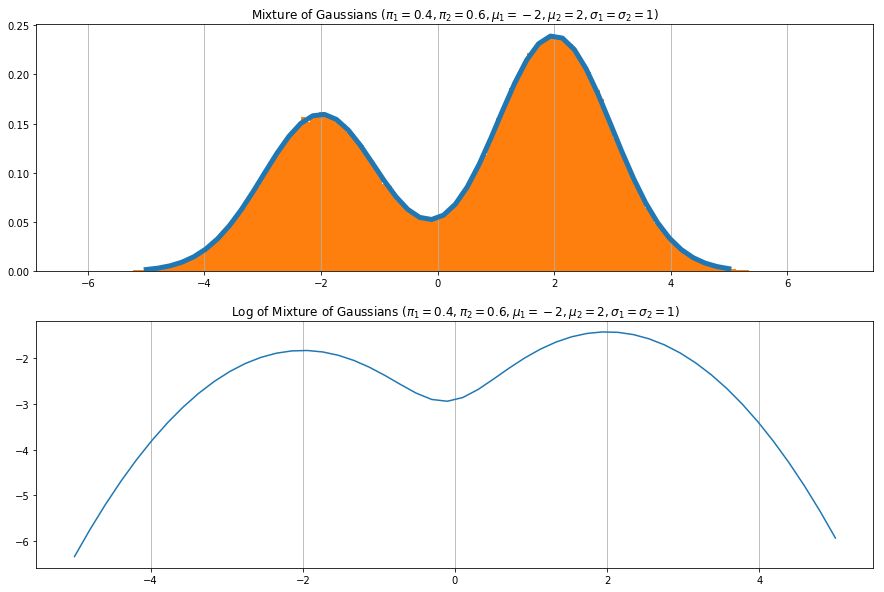
\includegraphics[height=0.7\textwidth]{mog.png}
\section{Frequentist methods}

\subsection{MAP}
In this case, we are interested in finding the solution to the following problem,
\begin{align}
\hat{\theta}_{MAP} = \argmaxA_{\theta} P(\theta \mid y_{1:N}) =  \argmaxA_{\theta} P(y_{1:N} \mid \theta) P(\theta). 
\end{align}
The problem with this approach is that we do not know $P(\theta)$. 

\subsection{MLE}
This is a simpler problem in which we have
\begin{align}
\hat{\theta}_{MLE} = \argmaxA_{\theta} P(y_{1:N} \mid \theta).
\end{align}
Due to the independence of the data points we can write
\begin{align}
\hat{\theta}_{MLE} &= \argmaxA_{\theta} P(y_{1:N} \mid \theta) = \argmaxA_{\theta} \prod_{i=1}^N P(y_i \mid \theta) \nonumber \\ 
&= \argmaxA_{\theta} \sum_{i=1}^N \log \left( P(y_i \mid \theta) \right).
\end{align}
 Finding the maximizing $\theta$ in this problem can be challenging. Trying to analytically solve the problem by taking the derivative is not possible since analytic solution does not exist. However, we can use gradient descent to estimate the parameter vector.  In gradient descent estimation we want to minimize
 \begin{align}
l (\theta)  &=  -\sum_{i=1}^N \log \left( P(y_i \mid \theta) \right) \nonumber \\ &= -\sum_{i=1}^N \log \left( \pi_1 \frac{1}{\sigma_1 \sqrt{2 \pi}} \exp \left( -\frac{(y_i-\mu_1)^2}{2\sigma_1^2}\right) + \pi_2 \frac{1}{\sigma_2 \sqrt{2 \pi}} \exp \left( -\frac{(y_i-\mu_2)^2}{2\sigma_2^2}\right) \right)  \nonumber 
\end{align}
with respect to parameters  $\theta = (\pi_1, \mu_1, \sigma_1, \pi_2, \mu_2, \sigma_2)$. We initialize by some random choice for these parameters and then iterate.  The problem with this method is that sometimes, gradient is hard to compute. 

\subsubsection{Expectation Maximization (EM)}
The EM algorithm attempts to find maximum likelihood estimates for models with latent variables. In the following, we will give a brief overview of the EM algorithm. We assume that the data $y$ is coming from a latent random variable $z$. Hence,
\begin{align}
f(\theta) &= \log \left( P(y \mid \theta) \right) = \log \left( \sum_z P(y,z \mid \theta)\right) \nonumber \\
&= \log \left( \sum_z q(z \mid y, \theta) \frac{P(y,z \mid \theta)}{q(z \mid y, \theta)}\right) \nonumber \\
&\ge \sum_z q(z \mid y, \theta) \log \left( \frac{P(y,z \mid \theta)}{q(z \mid y, \theta)} \right) \nonumber \\
&= \sum_z q(z \mid y, \theta) \log \left( \frac{P(z \mid y, \theta) P(y \mid \theta)}{q(z \mid y, \theta)} \right) \nonumber \\
&= - D_{KL}\left( q(z \mid y, \theta) ~ ||~ P(z \mid y, \theta) \right) + \log \left( P(y \mid \theta) \right).v 
\end{align}
Where $ q(z \mid y, \theta) $ is an arbitrary density over $z$ and the inequality is valid due to Jensen's inequality and concavity of the log function. Now, instead of maximizing $f(\theta)$ directly, one can maximize the lower bound, i.e.
\begin{align}
F(q, \theta) &\triangleq \sum_z q(z \mid y, \theta) \log \left( \frac{P(z \mid y, \theta) P(y \mid \theta)}{q(z \mid y, \theta)} \right) \nonumber \\
&= - D_{KL}\left( q(z \mid y, \theta) ~ ||~ P(z \mid y, \theta) \right) + \log \left( P(y \mid \theta) \right)
\end{align}
via coordinate ascent algorithm. This will be the EM algorithm with the following steps:
\begin{align}
\mathbf{E-Step} &: q^{(t+1)} = \argmaxA_{q} F(q, \theta^{(t)}) \\
\mathbf{M-Step} &: \theta^{(t+1)} = \argmaxA_{\theta} F(q^{(t+1)}, \theta).
\end{align}
Starting with some initial value of $\theta^{(0)}$, one can cycle between the E and M steps until $\theta^{(t)}$ converges to a local maximum. Computing the E step seem to be a pain in the ass since we are maximizing over the space of distributions. But notice that maximizing $F(q, \theta)$ over $q$ is equivalent to minimizing the KL distance between $q(z \mid y, \theta)$  and $P(z \mid y, \theta) $. Hence, 
\begin{align}
q^{(t+1)} = P(z \mid y, \theta^{(t)}).
\label{eq_q_t_1}
\end{align}
Notice that at this minimizing choice for KL distance, the lower bound becomes equal to the negative log likelihood function for $\theta^{(t)}$. 

So at this point, we don't need to worry about finding the optimal $q$ since we know it's exact form and we know that it is a distribution that depends on $\theta^{(t)}$. In M step, we fix $q$ and we note that
\begin{align}
F(q, \theta) &=  \sum_z q(z \mid y, \theta) \log \left( \frac{P(y,z \mid \theta)}{q(z \mid y, \theta)} \right) \nonumber \\
&= \sum_z q(z \mid y, \theta) \log \left( P(y,z \mid \theta)  \right) \nonumber \\
&- \sum_z q(z \mid y, \theta) \log \left(q(z \mid y, \theta) \right) \nonumber \\
&= \sum_z q(z \mid y, \theta) \log \left( P(y,z \mid \theta)  \right) + H(q),
\end{align}
where $H(q)$ is the entropy of $q$ and is not changing by $\theta$ in the M step as $q$ is fixed in the E step. Hence, maximizing $F(q, \theta)$ in the M step is equivalent to maximizing the expected complete log-likelihood function. In other words, if we define 
\begin{align}
Q(\theta \mid \theta^{(t)}) &\triangleq \sum_z q(z \mid y, \theta^{(t)}) \log \left( P(y,z \mid \theta)  \right) \nonumber \\
&=\mathbb{E}_{P(z \mid y, \theta^{(t)})} \left[ \log \left( P(y, z \mid \theta)\right)\right]
\end{align}
then using equation \eqref{eq_q_t_1}, we have 
\begin{align}
\argmaxA_{\theta}  F(q^{(t+1)}, \theta) &= \argmaxA_{\theta} F\left(P(z \mid y, \theta^{(t)}), \theta \right) = \argmaxA_{\theta} Q(\theta \mid \theta^{(t)}).
\end{align}
Therefore, in summary the EM algorithm can be summarized as follows
\begin{align}
\mathbf{E-Step} &: \mathrm{Compute}~ Q(\theta \mid \theta^{(t)}) =\mathbb{E}_{P(z \mid y, \theta^{(t)})} \left[ \log \left( P(y, z \mid \theta)\right)\right] \label{eq_e_step} \\
\mathbf{M-Step} &: \theta^{(t+1)} = \argmaxA_{\theta} \mathbb{E}_{P(z \mid y, \theta^{(t)})} \left[ \log \left( p (y, z \mid \theta) \right) \right].
\label{eq_m_step}
\end{align}
Now, back to our original problem, to generalize the problem to a mixture of $K$ Gaussians, let $z$ be a $K$-dimensional binary random variable which has a 1-of-$K$ representation in which a particular element $z^k$ is equal to 1 and all other elements are equal to 0. The values of $z^k$ therefore satisfy $z^k \in \{0, 1\}$ and $\sum_k z^k = 1$, and we see that there are $K$ possible states for the vector $z$ according to which element is nonzero. The marginal distribution over $z$ is specified in terms of the mixing coefficients $\pi_k$, such that $P(z^k = 1) = \pi_k$ and $0 \le \pi_k \le 1$ and $\sum_k \pi_k =1$. For the $i^{th}$ sample, we can write
\begin{align}
P(z_i \mid \theta) = \prod_{k=1}^K \pi_k^{z^k_i }.
\end{align}
Hence, 
\begin{align}
P(z_{1:N} \mid \theta) = \prod_{i=1}^N  \prod_{k=1}^K \pi_k^{z^k_i }.
\end{align}
similarly
\begin{align}
P(y_{1:N} \mid z_{1:N}, \theta ) = \prod_{i=1}^N  \prod_{k=1}^K \mathcal{N}(y_{i} ; \mu_k, \sigma_k)^{z^k_i}.
\end{align}
and 
\begin{align}
P(y_{1:N} , z_{1:N} \mid \theta ) = \prod_{i=1}^N  \prod_{k=1}^K (\pi_k \mathcal{N}(y_{i} ; \mu_k, \sigma_k))^{z^k_i}.
\end{align}
and 
\begin{align}
\log \left( P(y_{1:N} , z_{1:N} \mid \theta ) \right)= \sum_{i=1}^N  \sum_{k=1}^K z^k_i \log \left( \pi_k \mathcal{N}(y_{i} ; \mu_k, \sigma_k) \right).
\end{align}
Using Bayes rule, 
\begin{align}
P(z_{1:N} \mid y_{1:N}, \theta ) &= \frac{P(y_{1:N} \mid z_{1:N}, \theta ) P(z_{1:N} \mid \theta)}{\sum_z P(y_{1:N} \mid z_{1:N}, \theta ) P(z_{1:N} \mid \theta)}  \nonumber \\
&= \frac{\prod_{i=1}^N \prod_{k=1}^K ( \pi_k\mathcal{N}(y_i ; \mu_k, \sigma_k))^{z^k_i }}{\prod_{i=1}^N \sum_{j=1}^K \pi_j \mathcal{N}(y_i ; \mu_j, \sigma_j) } \nonumber \\
&=\prod_{i=1}^N   \frac{\prod_{k=1}^K ( \pi_k\mathcal{N}(y_i ; \mu_k, \sigma_k))^{z^k_i }}{\sum_{j=1}^K \pi_j \mathcal{N}(y_i ; \mu_j, \sigma_j) }.
\end{align}
Denoting $\gamma(z^k_i; y_i, \theta) \triangleq P(z^k_i = 1\mid y_i, \theta ) $, we have
\begin{align}
\gamma(z^k_i; y_i, \theta )  =   \frac{  \pi_k\mathcal{N}(y_i ; \mu_k, \sigma_k) }{\sum_{j=1}^K \pi_j \mathcal{N}(y_i ; \mu_j, \sigma_j) }.
\label{eq_gamma}
\end{align}
Since $z$ can only take discrete values, the E-Step in equation \eqref{eq_e_step} can be written as 
\begin{align}
Q(\theta \mid \theta^{(t)}) &= \mathbb{E}_{P(z_{1:N} \mid y_{1:N}, \theta^{(t)})} \left[ \log \left( P(y_{1:N}, z_{1:N} \mid \theta)\right)\right] \nonumber \\
&= \mathbb{E}_{P(z_{1:N} \mid y_{1:N}, \theta^{(t)})} \left[ \sum_{i=1}^N  \sum_{k=1}^K z^k_i \log \left( \pi_k \mathcal{N}(y_{i} ; \mu_k, \sigma_k) \right) \right] \nonumber \\
&= \sum_{i=1}^N  \sum_{k=1}^K \mathbb{E}_{P(z_{1:N} \mid y_{1:N}, \theta^{(t)})} \left[z^k_i \log \left( \pi_k \mathcal{N}(y_{i} ; \mu_k, \sigma_k) \right) \right] \nonumber \\
&= \sum_{i=1}^N  \sum_{k=1}^K \mathbb{E}_{P(z_{1:N} \mid y_{1:N}, \theta^{(t)})} \left[z^k_i \right] \log \left( \pi_k \mathcal{N}(y_{i} ; \mu_k, \sigma_k) \right)  \nonumber \\
&= \sum_{i=1}^N  \sum_{k=1}^K \mathbb{E}_{P(z_{i} \mid y_{i}, \theta^{(t)})} \left[z^k_i \right] \log \left( \pi_k \mathcal{N}(y_{i} ; \mu_k, \sigma_k) \right)  \nonumber \\
&= \sum_{i=1}^N \sum_{k=1}^K \gamma(z^k_i; y_i, \theta^{(t)} )  \log \left( \pi_k \mathcal{N}(y_i ; \mu_k, \sigma_k) \right)
\end{align}
and the M-Step in equation \eqref{eq_m_step} involves maximizing the above $Q(\theta \mid \theta^{(t)}) $ to find the parameters of the next iteration. Taking the derivative with respect to $\mu_k$ we have 
\begin{align}
\frac{\partial Q(\theta \mid \theta^{(t)})}{\partial \mu_k} &= 0 \Rightarrow  \sum_{i=1}^N  \gamma(z^k_i; y_i, \theta^{(t)} )   \left( \mu_k - y_i  \right) = 0. \nonumber
\end{align}
Therefore,
\begin{align}
\mu_k^{(t+1)} = \frac{1}{\sum_{i=1}^N  \gamma(z^k_i; y_i, \theta^{(t)}) } \sum_{i=1}^N  \gamma(z^k_i; y_i, \theta^{(t)})  y_i. 
\end{align}
Denoting 
\begin{align}
N_k \triangleq \sum_{i=1}^N  \gamma(z^k_i; y_i, \theta^{(t)}) ,
\label{eq_def_nk}
\end{align}
we have 
\begin{align}
\mu_k^{(t+1)} = \frac{1}{N_k } \sum_{i=1}^N  \gamma(z^k_i; y_i, \theta^{(t)})  y_i
\label{eq_update_mu}
\end{align}
Similarly, taking the derivative with respect to $\sigma_k$, we have 
\begin{align}
\frac{\partial Q(\theta \mid \theta^{(t)})}{\partial \sigma_k} &= 0 \Rightarrow  \sum_{i=1}^N  \gamma(z^k_i; y_i, \theta^{(t)} )   \left( \frac{(y_i - \mu_k)^2}{\sigma_k^2} - 1  \right) = 0. \nonumber
\end{align}
Plugging in $\mu_k = \mu_k^{(t+1)}$ we have 
\begin{align}
\sigma_k^{(t+1)} =  \sqrt{\frac{1}{N_k} \sum_{i=1}^N  \gamma(z^k_i; y_i, \theta^{(t)})  (y_i - \mu_k^{(t+1)})^2}. 
\label{eq_update_sigma}
\end{align}
It only remains to find $\pi_k^{(t+1)}$.  To find $\pi_k^{(t+1)}$, we should notice that $\sum_{k=1}^K \pi_k = 1$. Therefore, to optimize for $\pi_k$'s we need to add a Lagrange constraint to $Q(\theta \mid \theta^{(t)})$ when taking the derivative. Hence, we should maximize
\begin{align}
 L(\theta \mid \theta^{(t)})  \triangleq Q(\theta \mid \theta^{(t)}) + \lambda \left(\sum_{k=1}^K \pi_k -1 \right) \nonumber
\end{align}
Taking the derivative with respect to $\pi_k$'s we have 
\begin{align}
\frac{\partial L(\theta \mid \theta^{(t)})}{\partial \pi_k} &= \frac{\partial Q(\theta \mid \theta^{(t)})}{\partial \pi_k} + \lambda = \sum_{i=1}^N  \frac{\gamma(z^k_i; y_i, \theta^{(t)} )}{\pi_k} + \lambda = \frac{N_k}{\pi_k} + \lambda = 0 \Rightarrow \pi_k = \frac{N_k}{\lambda} \nonumber 
\end{align}
Since sum of all $\pi_k$'s should be one, we have 
\begin{align}
\sum_{k=1}^K \frac{N_k}{\lambda} = 1  \Rightarrow \lambda &= \sum_{k=1}^K  N_k = \sum_{k=1}^K \sum_{i=1}^N \gamma(z^k_i; y_i, \theta^{(t)} ) \nonumber \\
&=  \sum_{i=1}^N  \sum_{k=1}^K \gamma(z^k_i; y_i, \theta^{(t)} ) = \sum_{i=1}^N 1 = N \nonumber 
\end{align}
Therefore, 
\begin{align}
\pi_k^{(t+1)} = \frac{N_k}{N}. 
\label{eq_update_pi}
\end{align}
To summarize it all, the E-Step in mixture of Gaussians is equivalent to calculating $\gamma(z^k_i; y_i, \theta^{(t)} )$ based on equation \eqref{eq_gamma} and the M-Step is equivalent to updating the parameters based on equations \eqref{eq_def_nk}, \eqref{eq_update_mu}, \eqref{eq_update_sigma} and  \eqref{eq_update_pi}. These are pretty consistent with equations in page 439 of \cite{bishop2006pattern}.

\bibliographystyle{plain}
\bibliography{mog_bib}
\end{document}